\chapter{Costo de la solución}

El presente capítulo estima el costo de implementación del prototipo propuesto.
El análisis considera los componentes electrónicos principales, los materiales de
fabricación y los elementos de ensamblaje necesarios para construir un sistema
inteligente de control ESD de bajo costo. Los precios utilizados corresponden a
valores de referencia obtenidos de proveedores comerciales en línea consultados en
amazon.com el 29 de julio del 2026, únicamente con fines de estimación económica.

Amazon.com se utiliza en este capítulo como una referencia comercial para
comparar costos aproximados, y no como fuente técnica para la selección,
caracterización o validación de los componentes del sistema. Las especificaciones
técnicas, criterios de funcionamiento y parámetros de diseño se fundamentan en
hojas de datos, manuales de fabricante, normas ESD y documentación técnica
especializada. Por lo tanto, los valores económicos presentados pueden variar
según disponibilidad, proveedor, impuestos, envío y fecha de compra.

\section{Estimación de costos de hardware}

La Tabla~\ref{tab:presupuesto_hardware} presenta los principales módulos
electrónicos seleccionados para la implementación del prototipo. Estos
componentes corresponden a los subsistemas de verificación ESD, identificación
de usuario, interfaz gráfica, monitoreo ambiental, almacenamiento y alimentación
del sistema.

\begin{table}[H]
\centering
\caption{Estimación de costos de los componentes electrónicos principales.}
\label{tab:presupuesto_hardware}
\begin{tabular}{p{5.2cm} c c c}
\toprule
\textbf{Componente} &
\textbf{Cantidad} &
\textbf{Costo unitario (USD)} &
\textbf{Subtotal (USD)} \\
\midrule

Probador HZR-171 para pulsera antiestática &
1 & 29.99 & 29.99 \\

ESP32-WROOM-32 &
1 & 8.99 & 8.99 \\

Pantalla HMI ESP32 de 7 pulgadas &
1 & 59.99 & 59.99 \\

Lector de código de barras GM67 &
1 & 21.99 & 21.99 \\

Módulo ESP32-S3 CAM &
1 & 22.95 & 22.95 \\

Módulo SHT31-D de temperatura y humedad &
1 & 8.49 & 8.49 \\

Módulo convertidor DC-DC XL6019 &
1 & 7.19 & 7.19 \\

Parlante de 8 $\Omega$, 3 W &
1 & 4.99 & 4.99 \\

Memoria microSD de 32 GB &
1 & 13.99 & 13.99 \\

Módulo USB-C PD &
1 & 9.59 & 9.59 \\

Módulo RTC DS3231 &
1 & 4.00 & 4.00 \\

\midrule
\textbf{Subtotal de hardware} &
& & \textbf{192.16} \\
\bottomrule
\end{tabular}
\end{table}

La memoria microSD de 32 GB se selecciona para almacenar los registros históricos
y los reportes generados por el sistema. Aunque los archivos de reporte en
formato CSV requieren poco espacio de almacenamiento, se selecciona esta
capacidad debido a que para la fecha de este anteproyecto el precio de una memoria SD 
de 32 GB es equivalente a alguna de menor capacidad, esta información se obtiene de 
la tienda en línea amazon.com.

\section{Costos de fabricación y ensamblaje}

Además de los módulos electrónicos principales, se consideran materiales de
fabricación para la interconexión, montaje y construcción física del prototipo.
Estos elementos se agrupan en categorías generales debido a que corresponden a
materiales de bajo costo, tales como cables, conectores, placas de prototipado,
tornillería y consumibles de impresión 3D.

\begin{table}[H]
\centering
\caption{Estimación de costos de fabricación y ensamblaje.}
\label{tab:presupuesto_fabricacion}
\begin{tabularx}{\textwidth}{X X c}
\toprule
\textbf{Concepto} &
\textbf{Descripción} &
\textbf{Costo estimado (USD)} \\
\midrule

Cableado eléctrico &
Cable 24 AWG para interconexión interna~ &
9.00 \\

Placas FR4 de prototipado &
Placas FR4 de 10 cm $\times$ 15 cm~ &
13.19 \\

Material de impresión 3D &
Consumo aproximado de 500 g de PLA~ &
5.70 \\

Materiales mecánicos menores &
Tornillos, separadores, conectores, termocontraíble y otros consumibles &
20.00 \\

\midrule
\textbf{Subtotal de fabricación y ensamblaje} &
&
\textbf{47.89} \\
\bottomrule
\end{tabularx}
\end{table}

No se incluye el costo de herramientas o equipos ya disponibles, tales como
impresora 3D, estación de soldadura, computadora de desarrollo, multímetro,
instrumentos de medición o licencias de software. Estos recursos forman parte
de la infraestructura disponible para la ejecución del proyecto y no
corresponden a materiales consumibles del prototipo.

\section{Costo total estimado del prototipo}

A partir de los costos de hardware, fabricación y ensamblaje, se obtiene el
costo total estimado mostrado en la Tabla~\ref{tab:presupuesto_total}. Este
valor representa el costo directo de los materiales necesarios para la
construcción del prototipo funcional.

\begin{table}[H]
\centering
\caption{Costo total estimado del prototipo.}
\label{tab:presupuesto_total}
\begin{tabular}{p{8cm} c}
\toprule
\textbf{Categoría} & \textbf{Costo estimado (USD)} \\
\midrule

Componentes electrónicos principales & 192.16 \\
Materiales de fabricación y ensamblaje & 47.89 \\

\midrule
\textbf{Costo total estimado} & \textbf{240.05} \\
\bottomrule
\end{tabular}
\end{table}

A partir del costo directo calculado de 240.05 USD, se establece un presupuesto
de referencia de \textbf{300 USD}. La diferencia se reserva para cubrir posibles
variaciones de precio, costos de envío y materiales menores que puedan
requerirse durante el ensamblaje.

\section{Comparación con soluciones comerciales}

Uno de los objetivos principales del proyecto es desarrollar una solución de
bajo costo en comparación con sistemas comerciales de control ESD. La
Figura~\ref{fig:comparacion_grafica_costos} presenta una comparación entre el costo
estimado del prototipo y diferentes soluciones comerciales analizadas en el
estado del arte.

Esta comparación se utiliza únicamente como referencia económica, debido a que
los equipos comerciales pueden incluir funciones adicionales, certificados de
calibración, accesorios y servicios de soporte que no forman parte del alcance
del prototipo
\cite{SCS_770758,PGT120,PGT130DT,SmartLogPro2}. Por lo tanto, los valores
presentados no establecen una equivalencia directa entre las soluciones.

\begin{figure}[H]
\centering
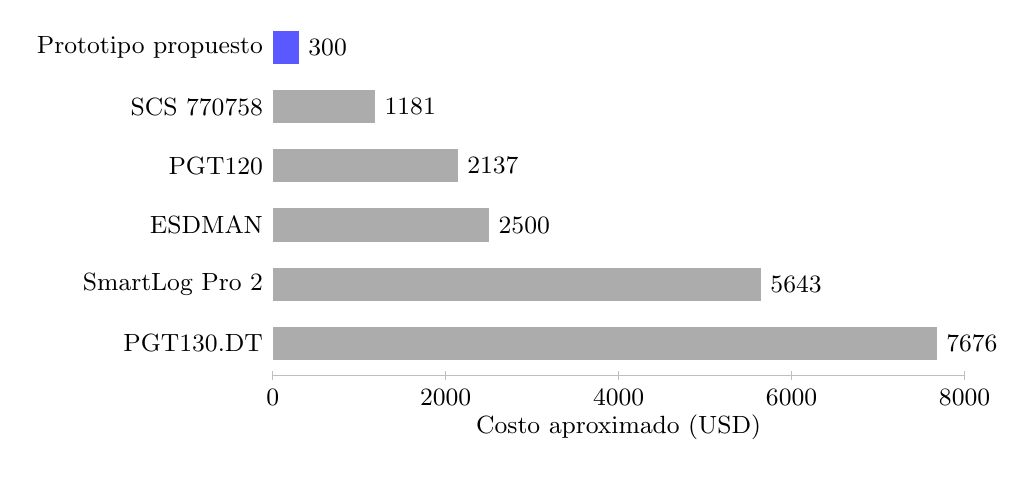
\begin{tikzpicture}[x=0.0011cm,y=0.75cm,font=\small]
    \draw[gray!50] (0,-0.55) -- (8000,-0.55);
    \foreach \x in {0,2000,4000,6000,8000} {
        \draw[gray!50] (\x,-0.62) -- (\x,-0.48);
        \node[below] at (\x,-0.62) {\x};
    }
    \node[below] at (4000,-1.05) {Costo aproximado (USD)};

    \node[anchor=east] at (0,5) {Prototipo propuesto};
    \fill[blue!65] (0,4.72) rectangle (300,5.28);
    \node[anchor=west] at (300,5) {300};

    \node[anchor=east] at (0,4) {SCS 770758};
    \fill[gray!65] (0,3.72) rectangle (1181,4.28);
    \node[anchor=west] at (1181,4) {1181};

    \node[anchor=east] at (0,3) {PGT120};
    \fill[gray!65] (0,2.72) rectangle (2137,3.28);
    \node[anchor=west] at (2137,3) {2137};

    \node[anchor=east] at (0,2) {ESDMAN};
    \fill[gray!65] (0,1.72) rectangle (2500,2.28);
    \node[anchor=west] at (2500,2) {2500};

    \node[anchor=east] at (0,1) {SmartLog Pro 2};
    \fill[gray!65] (0,0.72) rectangle (5643,1.28);
    \node[anchor=west] at (5643,1) {5643};

    \node[anchor=east] at (0,0) {PGT130.DT};
    \fill[gray!65] (0,-0.28) rectangle (7676,0.28);
    \node[anchor=west] at (7676,0) {7676};
\end{tikzpicture}
\caption{Comparación entre el presupuesto del prototipo y los precios
aproximados de las soluciones comerciales consultadas. Fuente: elaboración
propia a partir de
\cite{SCS_770758,PGT120,ESDMAN_0016809,SmartLogPro2,PGT130DT}.}
\label{fig:comparacion_grafica_costos}
\end{figure}

La Figura~\ref{fig:comparacion_grafica_costos} permite observar la diferencia
entre el presupuesto del prototipo y los precios de las soluciones comerciales
consultadas. Incluso la alternativa comercial de menor costo presenta un valor
cercano a cuatro veces el presupuesto estimado del prototipo.

\section{Análisis económico}

El presupuesto estimado muestra que es posible implementar las funciones
propuestas con un costo aproximado de 300 USD. Además, este valor se mantiene
por debajo del límite de 350 USD establecido como requerimiento no funcional
del proyecto.

Además del costo, la solución propuesta ofrece la ventaja de ser personalizable.
El sistema puede adaptarse a requerimientos específicos del laboratorio, como
el formato de registro, la interfaz de usuario, los métodos de identificación
y las condiciones de validación.

Los resultados indican que el prototipo puede construirse con un presupuesto
menor que el precio de las soluciones comerciales consultadas. Aunque no se
plantea como un sustituto directo de un equipo industrial certificado,
representa una alternativa viable para desarrollar y validar las funciones
definidas dentro del alcance académico del proyecto.
